\chapter{Results \& Analysis}
\label{ch:res}
The models described in the previous section were then simulated in \cite{cfx}. Note, refer to \hyperlink{appendixa}{Appendix A} for all CFX results.

%-----------------------------------------------------------------------------------------------------------------
\section{Convergence}
\label{sec:convg}

To monitor each models performance on the convergence of the previously defined $\delta_{r_{MAX}}$, convergence plots were exported (see Figures~\ref{fig:ref_convg}, \ref{fig:mod1_convg}, \ref{fig:mod2_convg}).

\begin{figure}[H]
	\centering
	\includegraphics[height=0.425\textheight,keepaspectratio]{ref/convergence}
	\caption{Reference model convergence.}
	\label{fig:ref_convg}
\end{figure}
\begin{figure}[H]
	\centering
	\includegraphics[height=0.425\textheight,keepaspectratio]{model1/convergence}
	\caption{Model 1 convergence.}
	\label{fig:mod1_convg}
\end{figure}
\begin{figure}[H]
	\centering
	\includegraphics[height=0.425\textheight,keepaspectratio]{model2/convergence}
	\caption{Model 2 convergence.}
	\label{fig:mod2_convg}
\end{figure}

Summarizing the above, the models converged in $i_{ref}=39$, $i_1=36$, and $i_2=44$ for the reference, model 1 and model 2, respectively. It is also clear that converge for reference and model 1 were rather smooth (see Figures~\ref{fig:ref_convg}, \ref{fig:mod1_convg}). Meanwhile, model 2 (see Figure~\ref{fig:mod2_convg}) has some very small oscillation. This is likely due to the nozzle air entering the mixing chamber in the opposite direction as the axial inlet causing more disorder.

%-----------------------------------------------------------------------------------------------------------------
\section{Validation}
\label{sec:valid}
The reference model is validated by comparing the CFX results to the experimental data from \cite{art}. Velocity $u-v$ and turbulent kinetic energy $k$ data at collected at $X^*=-0.87,\ 0,\ 1.6,\ 2.5,\ 4,\ 9$ are compared in the following plots.\\

Both simulated and experimental velocity $u$, $v$ and $k$ profiles at various $X^*$ are shown below in Figure~\ref{fig:exp_ref_u}, \ref{fig:exp_ref_v}, \ref{fig:exp_ref_k}. Note, see \hyperlink{appendixb}{Appendix B} for \cite{matlab} script used to create all of the foregoing plots.\\
\begin{figure}[H]
	\centering
	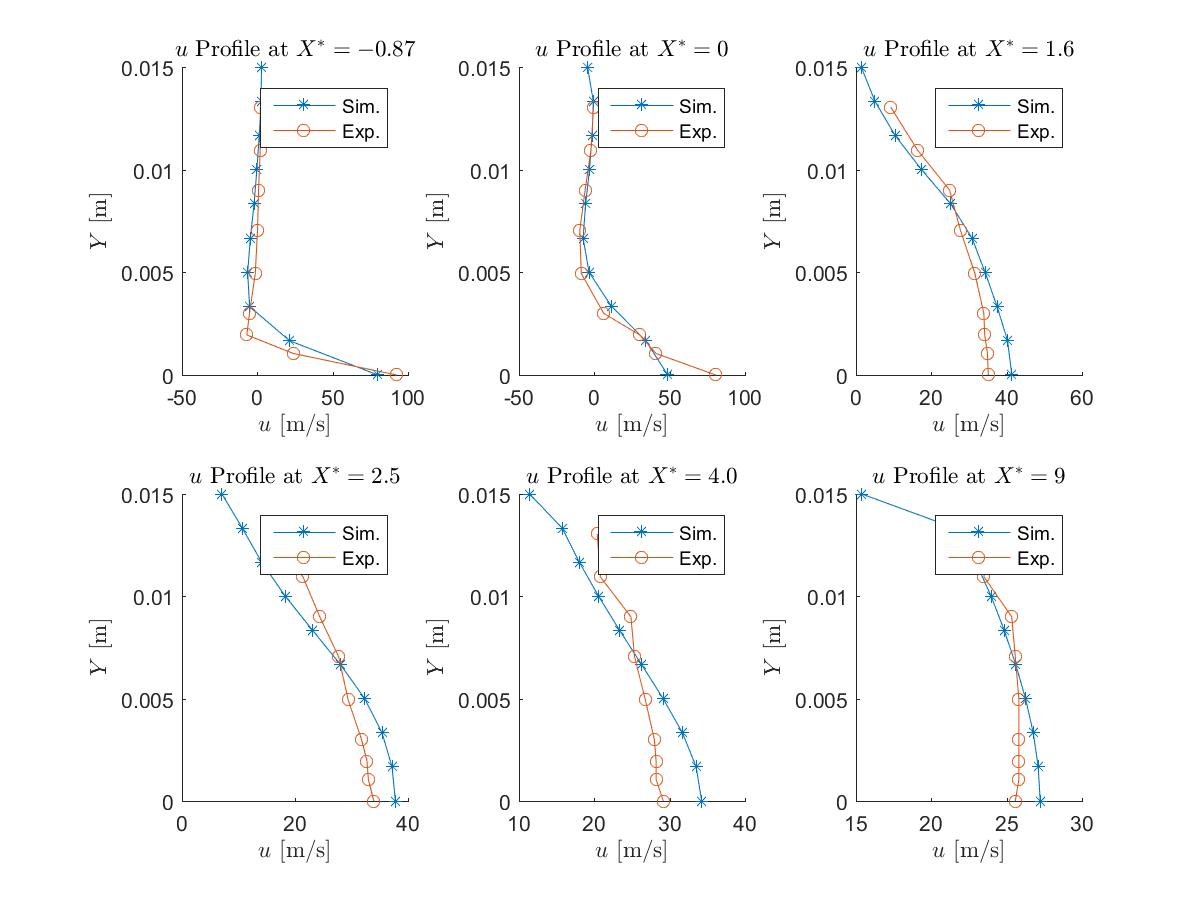
\includegraphics[height=0.425\textheight,keepaspectratio]{matlab/exp_ref_u}
	\caption{Comparison of experimental and simulated $u$ profiles at various $X^*$.}
	\label{fig:exp_ref_u}
\end{figure}

\begin{figure}[H]
	\centering
	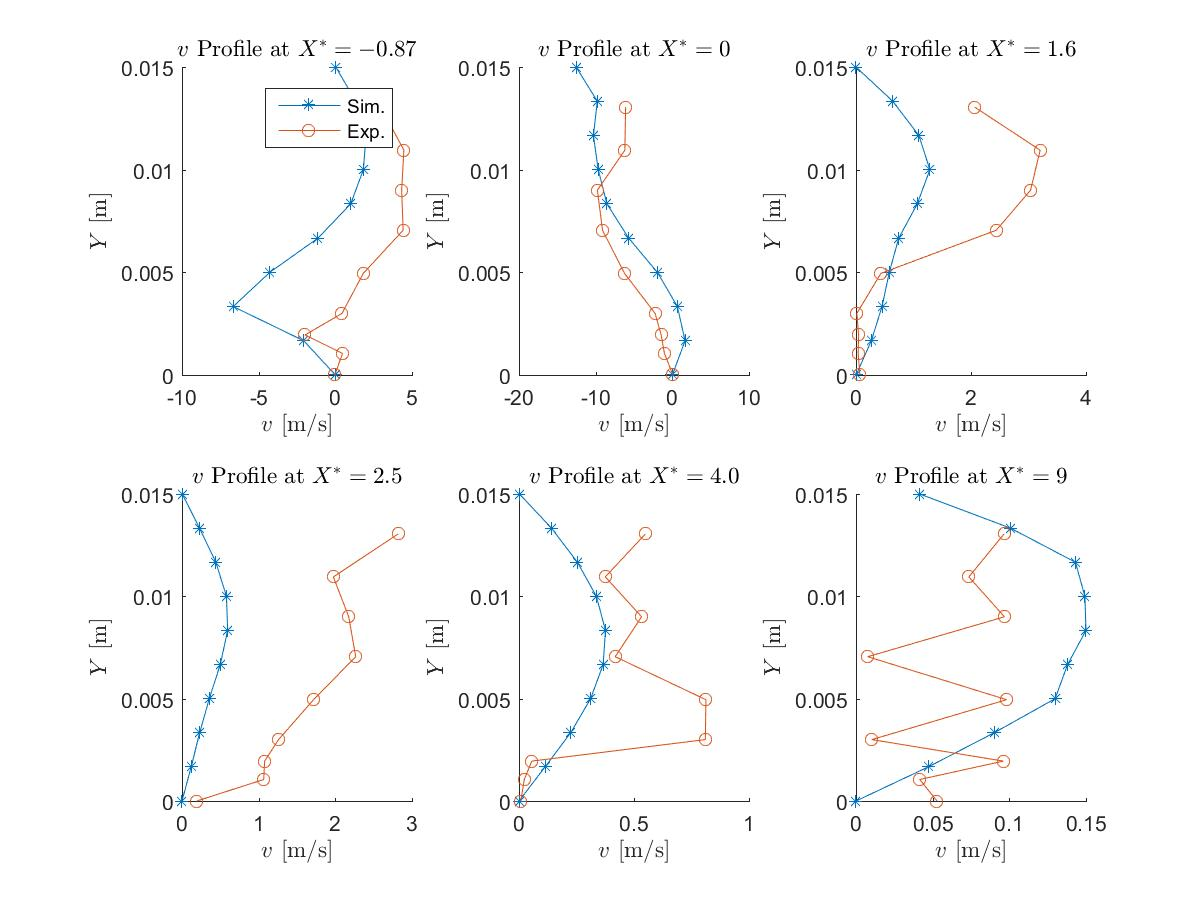
\includegraphics[height=0.425\textheight,keepaspectratio]{matlab/exp_ref_v}
	\caption{Comparison of experimental and simulated $v$ profiles at various $X^*$.}
	\label{fig:exp_ref_v}
\end{figure}

\begin{figure}[H]
	\centering
	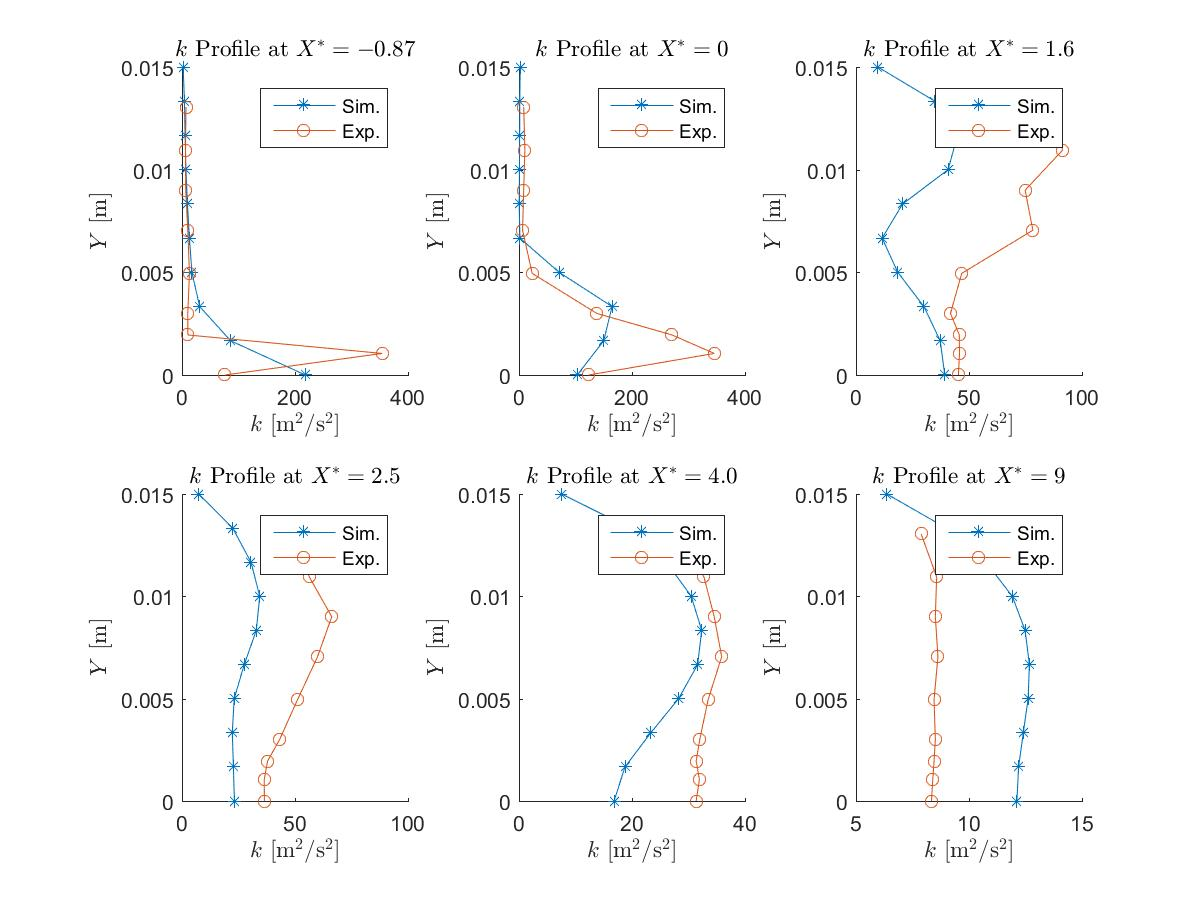
\includegraphics[height=0.425\textheight,keepaspectratio]{matlab/exp_ref_k}
	\caption{Comparison of experimental and simulated $k$ profiles at various $X^*$.}
	\label{fig:exp_ref_k}
\end{figure}

The simulated $u$ profiles match very well with experimental data for low $X^*$ (see Figure  \ref{fig:exp_ref_u}). Near the end of the domain, it appears that the discrepancies between data are larger.\\

As for both $v$ and $k$ profiles (Figures \ref{fig:exp_ref_v} and \ref{fig:exp_ref_k}) the simulation data does not compare very well with that of \cite{art}.\\

Possible causes for these differences could be to highly idealized simulation boundary conditions. Furthermore experimental measurement error is also highly likely. This clearly depicted in the $v$ profile at $X^*=9$ (see Figure~\ref{exp_ref_v}).
%-----------------------------------------------------------------------------------------------------------------
\section{Effects of Side Inlets}
\label{sec:effects_side}
The effect of .\\

Simulated $u$, $v$ and $k$ profiles for all models at various $X^*$ are shown below in Figures~\ref{fig:sim_compu} - \ref{fig:sim_compk}, respectively.
\begin{figure}[H]
	\centering
	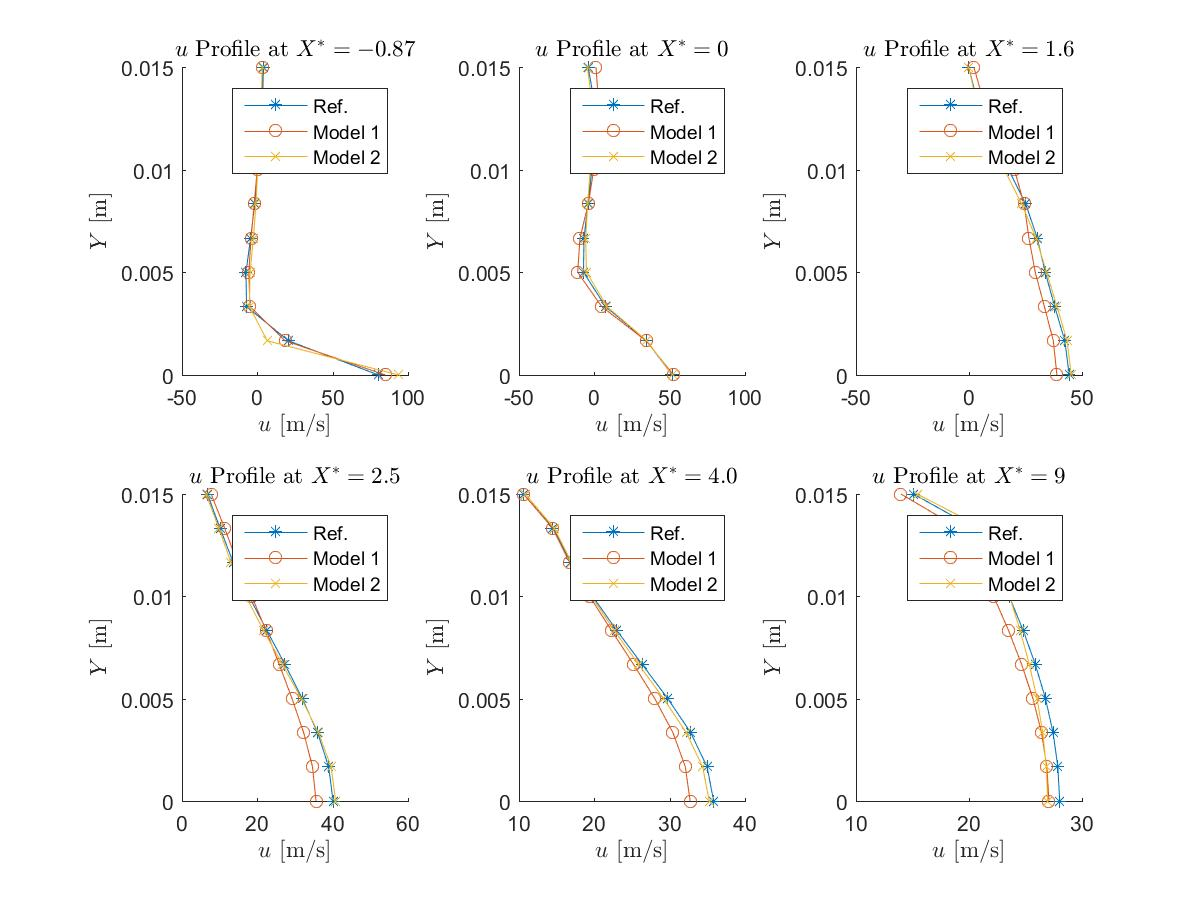
\includegraphics[height=0.425\textheight,keepaspectratio]{matlab/sim_compu}
	\caption{Comparison of all simulated $u$ profiles at various $X^*$.}
	\label{fig:sim_compu}
\end{figure}

\begin{figure}[H]
	\centering
	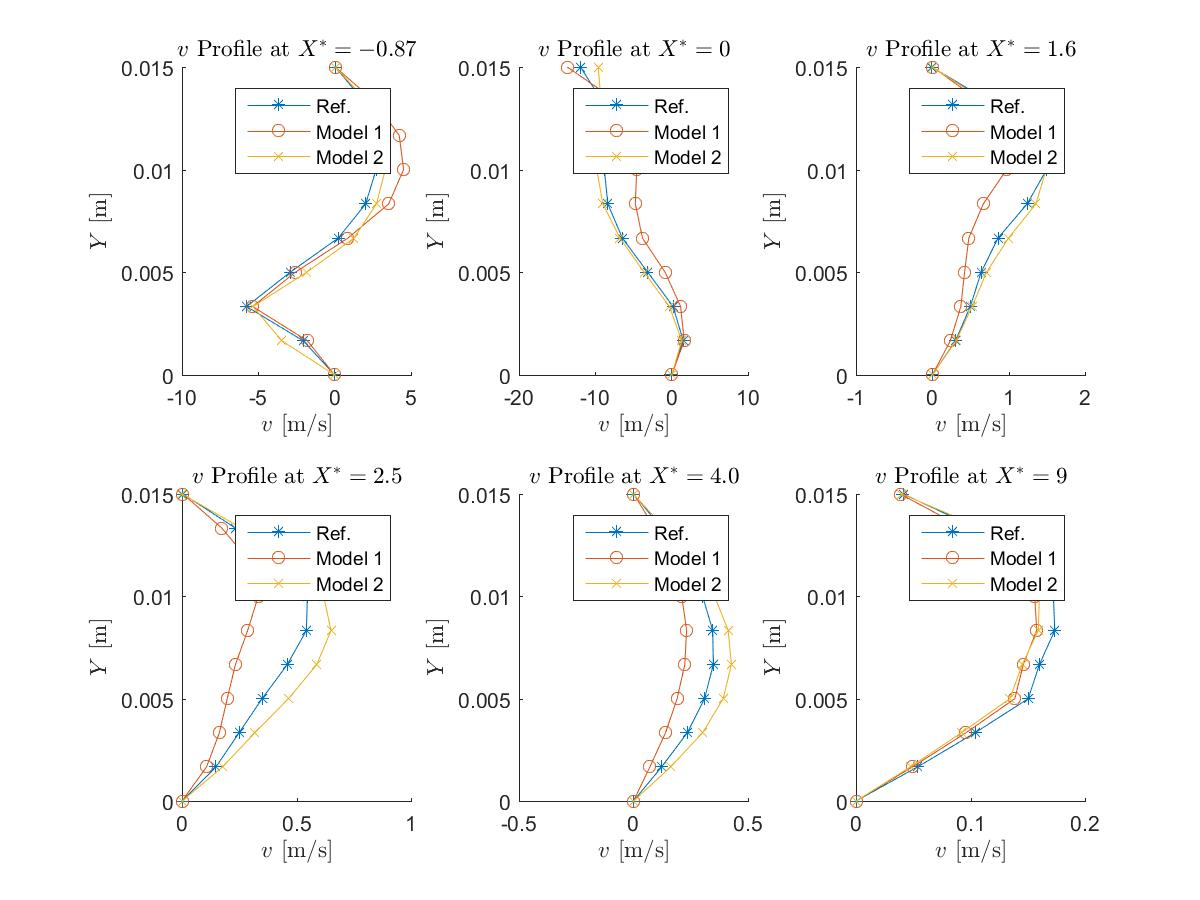
\includegraphics[height=0.425\textheight,keepaspectratio]{matlab/sim_compv}
	\caption{Comparison of all simulated $v$ profiles at various $X^*$.}
	\label{fig:sim_compv}
\end{figure}

\begin{figure}[H]
	\centering
	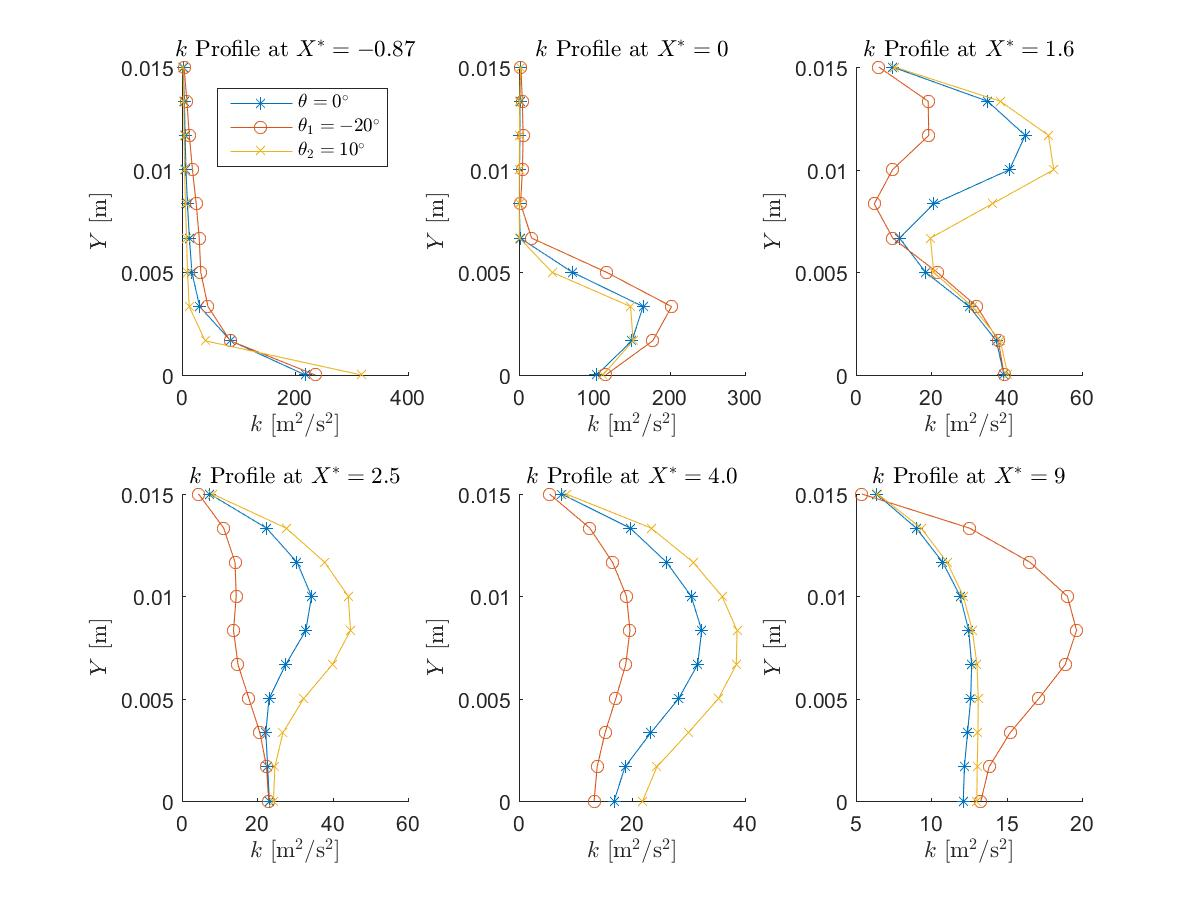
\includegraphics[height=0.425\textheight,keepaspectratio]{matlab/sim_compk}
	\caption{Comparison of all simulated $k$ profiles at various $X^*$.}
	\label{fig:sim_compk}
\end{figure}

Based on results from Figure \ref{fig:sim_compu}, there is hardly any variation in simulated $u$ profiles.\\

In Figures \ref{fig:sim_compv} and \ref{fig:sim_compk}, minimal variation is seen in both $v$ and $k$ profiles for $X^* \leq 0$ however, larger discrepancies are observed as $X^* \rightarrow 9$.\\

In Figure \ref{fig:sim_compT} below, temperature $T$ profiles are shown.
\begin{figure}[H]
	\centering
	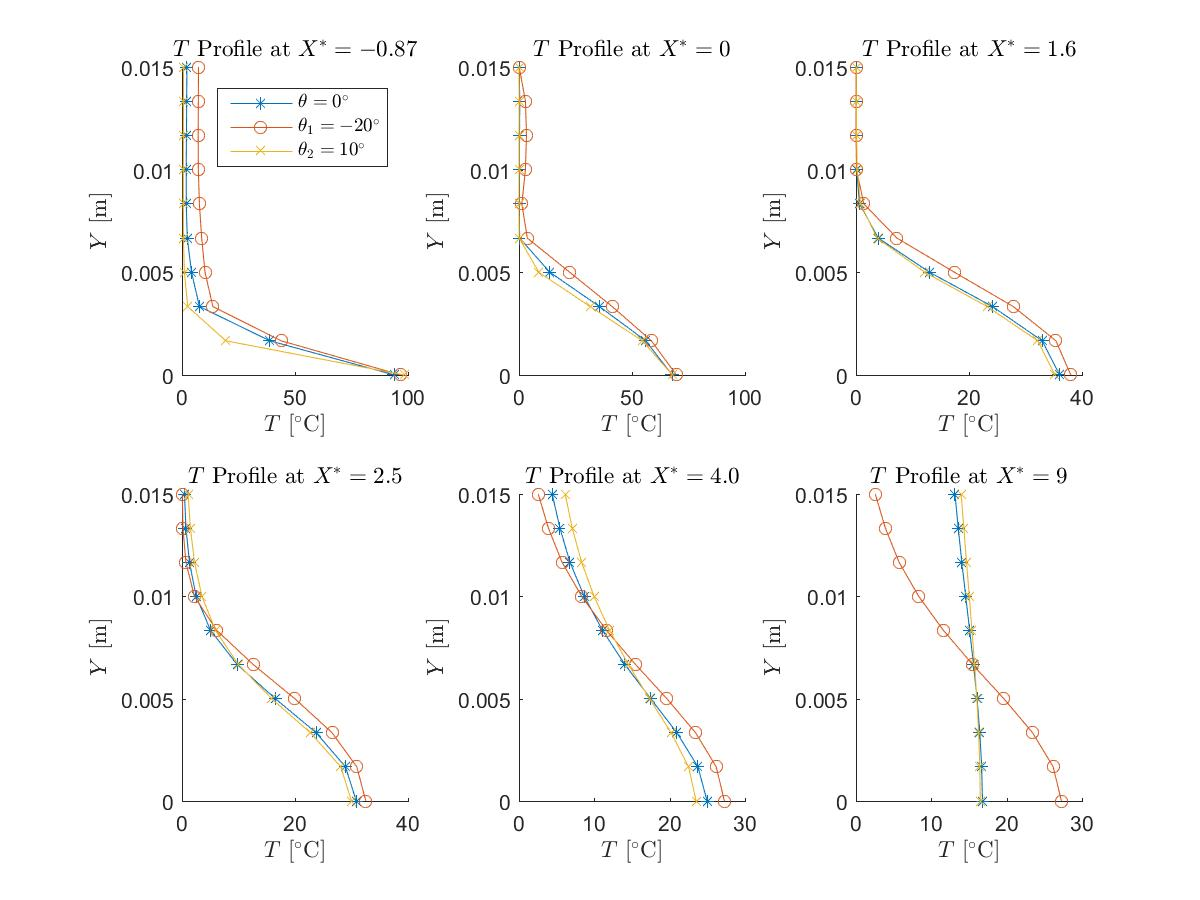
\includegraphics[height=0.425\textheight,keepaspectratio]{matlab/sim_compT}
	\caption{Comparison of all simulated $T$ profiles at various $X^*$.}
	\label{fig:sim_compT}
\end{figure}

Again as seen above, only a slight variation is seen between temperature profiles.\\

Observations from above are investigated below in Figure~\ref{fig:sim2_comp_T} where $T$ is plotted along $X^*$ at $Y^*=0$.
\begin{figure}[H]
	\centering
	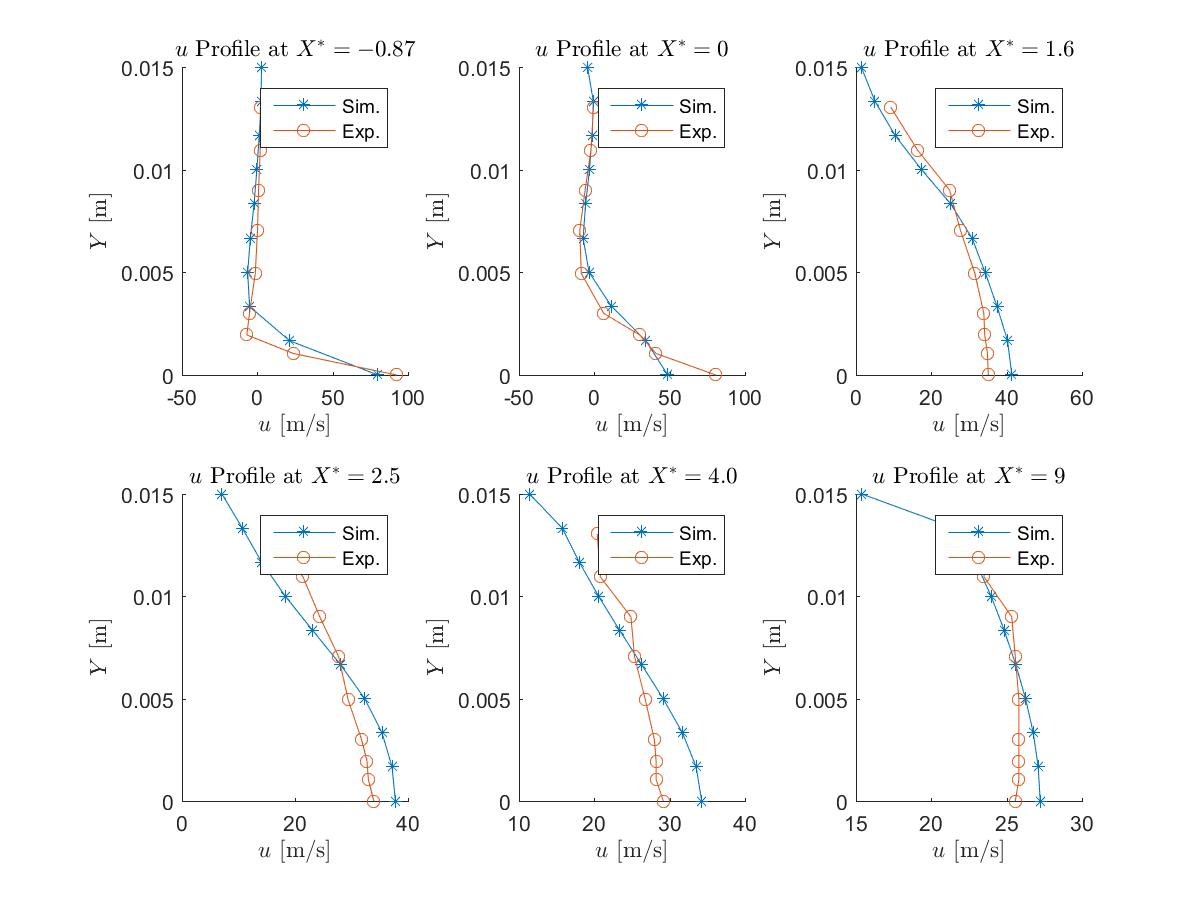
\includegraphics[scale=0.35]{matlab/sim2_comp_T}
	\caption{Variation of $T$ along $X^*$ at $Y^*=0$.}
	\label{fig:sim2_comp_T}
\end{figure}

Axially, it appears as though a CCW angle of 20 \textsuperscript{o} shows a higher temperature as $X^* \rightarrow 9$ indicating the best mixing of all three models.

%-----------------------------------------------------------------------------------------------------------------
\section{Comparison}
\label{sec:comp}

From \cite{mobin}, it appeared as though optimal mixing was observed for a CW angle of 20 \textsuperscript{o}.\\


Similarly, best mixing was observed for a XXX \textsuperscript{o}m \cite{curtis}.\\

Finally, \cite{tolu} saw a more uniform temperature mix for XXX \textsuperscript{o}.
 
%-----------------------------------------------------------------------------------------------------------------
\section{Source of Errors}
\label{sec:err}

As with many CFD simulations, there is a plethora of error which must be considered and understood. Errors in the physical modelling such as the geometry, the equations of state and turbulence model all effect the final solution. For these CFX simulations, the majority of the error is found in the turbulence model. \textbf{talk about why k-e is bad and others are better, Use of this model is further validated there are no curved surfaces nor rotating flows }\\

%Physical model \\
%-geometric model\\
%-equations of state\\
%-turbulence model\\
%
%
%Numerical model\\
%-discretization \\
%*differencing sceheme\\
%*grid resolution\\
%* cell shape\\\
%\\
%-solver\\
%*round off error

Furthermore, the selected numerical models also play a large role in error, primairly through discretization. For example, even though a high resolution scheme is selected due to its high accuracy in CFX, it is still only second order accurate or $\mathcal{O} (\Delta x^2)$ \cite{cfdbook}. \textbf{Also, the grid resolution error caused by the use of tri elements}. Other sources of numerical error are also attributed to the computer's round off.

